\documentclass[12pt]{extarticle}

\usepackage{tabularx}
\usepackage{amsmath}
\usepackage{extsizes}
\usepackage{graphicx}
\usepackage{amssymb}
\usepackage[english,russian]{babel}
\usepackage[utf8]{inputenc}
\usepackage[a4paper]{geometry}
\geometry{top=20mm,bottom=30mm,left=20mm,right=15mm}
\usepackage[T1,T2A]{fontenc}
\usepackage{setspace}
\usepackage{indentfirst}
\usepackage{caption}
\renewcommand{\baselinestretch}{1.5}
\usepackage{spverbatim}
\usepackage{listings}
\usepackage{xcolor}
\usepackage{tabularray}

\definecolor{codebg}{gray}{0.96}
\definecolor{comment}{gray}{0.45}
\definecolor{keyword}{RGB}{0, 75, 150}
\definecolor{string}{RGB}{150, 80, 30}
\definecolor{number}{gray}{0.5}
\definecolor{identifier}{rgb}{0,0,0}

\lstdefinestyle{coolprint}{
  basicstyle   = \ttfamily\footnotesize,
  keywordstyle = \bfseries\color{keyword},
  commentstyle = \itshape\color{comment},
  stringstyle  = \color{string},
  identifierstyle = \color{identifier},
  backgroundcolor = \color{codebg},
  numbers      = left,
  numberstyle  = \footnotesize\color{number},
  numbersep    = 5pt,
  frame        = single,
  framerule    = 0.8pt,
  framesep     = 3pt,
  breaklines   = true,
  breakatwhitespace = true,
  tabsize      = 4,
  showspaces   = false,
  showstringspaces = false,
  showtabs     = false,
  xleftmargin  = 10pt,
  xrightmargin = 5pt,
  aboveskip    = \medskipamount,
  belowskip    = \medskipamount,
  captionpos   = b,
}
\lstset{style=coolprint}

\begin{document}

\begin{center}
  \textbf{МИНОБРНАУКИ РОССИИ} \\
  \textbf{Санкт-Петербургский государственный} \\
  \textbf{электротехнический университет} \\
  \textbf{«ЛЭТИ» им. В.И. Ульянова (Ленина)} \\
  \textbf{Кафедра ВТ} \\
\end{center}

\vspace{0.25\textheight}

\begin{center}
\textbf{ОТЧЕТ} \\
\textbf{по лабораторной работе №2} \\
\textbf{по дисциплине «ОргЭВМиС»} \\
\textbf{Тема: КОМПИЛЯЦИЯ ПРОГРАММ НА ЯЗЫКЕ C И ВНУТРЕННЕЕ ПРЕДСТАВЛЕНИЕ ДАННЫХ В RIPES} \\
\end{center}

\vspace*{\fill}

\begin{center}
\begin{tabularx}{\textwidth}{ l X r }
 Студенты гр. 5352 & \rule{8cm}{0.2mm} & Cоболевский М.А. \\
 & \rule{8cm}{0.2mm} & Решетников С.А. \\
 Преподаватель & \rule{8cm}{0.2mm} & Кочетков А.В. \\
\end{tabularx}
\end{center}

\vspace{3em}

\begin{center}
Санкт-Петербург\\
\the\year
\end{center}

\thispagestyle{empty}

\pagebreak

\section{Задание на лабораторную работу}

Тип данных для вывода: \texttt{signed long}

Способ получения данных: Инициализация константы

\section{Текст программы}

\renewcommand{\baselinestretch}{1}
\begin{lstlisting}[language=C]
#include <stdio.h>
#include <limits.h>

void bits(long y)
{
    unsigned long x = y;
    const long nbits = sizeof y*8;
    for (int i = 0; i < nbits; ++i) {
        printf("%c", "01"[(x>>(nbits - i - 1))&1]);
    }
    printf("\n");
}

int main(void)
{
    const long konst = 0xfa55bea7;
    int i;
    printf("%p: %ld\n", (void *)&konst, konst);
    printf("LONG_MAX = %ld\n", LONG_MAX);
    printf("LONG_MIN = %ld\n", LONG_MIN);
    
    for (i = 0; i < sizeof konst; ++i)
        printf("%02x ", ((unsigned char *)&konst)[i]);
    printf("\n");
    bits(konst);
    
    return 0;
}\end{lstlisting}

\renewcommand{\baselinestretch}{1.5}

\section{Примеры запуска программ и снимки экрана}

Вывод запуска примера (константа \texttt{= 0xfa55bea7}):

\renewcommand{\baselinestretch}{1}
\begin{spverbatim}
0x7fffffd8: -95043929
LONG_MAX = 2147483647
LONG_MIN = -2147483648
a7 be 55 fa
11111010010101011011111010100111
\end{spverbatim}
\renewcommand{\baselinestretch}{1.5}

Данные в стеке (константа сохранена по адресу \texttt{0x7fffffd8}):

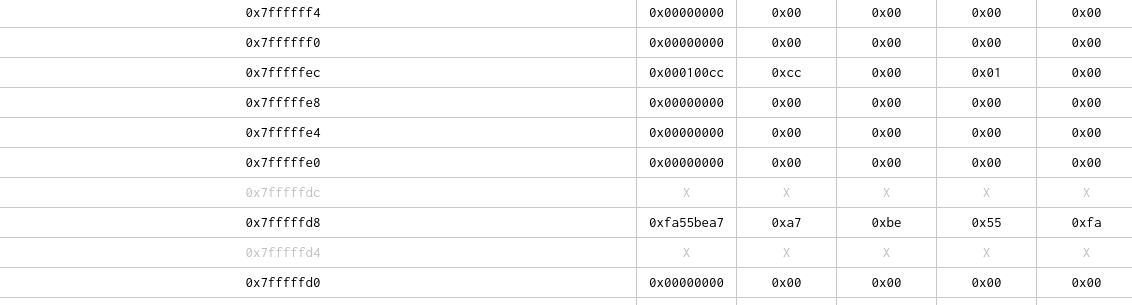
\includegraphics[width=\textwidth]{assets/2026-09-28-180207_1132x305_scrot.png}


\section{Выводы}

В ходе лабораторной работы мы ознакомились с процессом компиляции программ на языке C для архитектуры RISC-V и их запуском в симуляторе Ripes, а также изучили внутреннее представление данных.

Для выполнения пункта 2 были предприняты следующие действия: установлен и настроен симулятор Ripes с поддержкой RISC-V GCC; в настройках проекта указан компилятор \texttt{riscv64-unknown-elf-gcc} и необходимые флаги; подключены стандартные библиотеки C (libc, libm) и заголовочные файлы. После этого программы на C успешно компилировались и запускались.

В соответствии с вариантом задания (тип данных \texttt{signed long}, способ получения — инициализация константы) была написана программа, которая:
\begin{itemize}
    \item выводит значение константы \texttt{konst = 0xfa55bea7} в десятичном и шестнадцатеричном виде;
    \item выводит максимальное и минимальное значения типа \texttt{long} из файла \texttt{limits.h};
    \item побайтово отображает внутреннее представление константы в памяти;
    \item выводит двоичное представление числа.
\end{itemize}

Анализ результатов показал, что в среде Ripes тип \texttt{long} занимает 4 байта (32 бита), а не 8 байт, как на большинстве современных платформ. Это подтверждается значениями \texttt{LONG\_MAX = 2147483647} и \texttt{LONG\_MIN = -2147483648}. Константа \texttt{0xfa55bea7} интерпретируется как знаковое число \texttt{-95043929}. В памяти она хранится в порядке little-endian: байты \texttt{a7 be 55 fa}. Двоичное представление соответствует дополнительному коду для отрицательного числа.

В процессе работы были выявлены следующие особенности и возможные ошибки:
\begin{itemize}
    \item при использовании формата \texttt{\%ld} для \texttt{long} в Ripes (32-битная платформа) необходимо быть внимательным, так как размер \texttt{long} может отличаться от привычного;
    \item для вывода адреса переменной требуется приведение к \texttt{void *} и формат \texttt{\%p}, что и было сделано;
    \item стандартные библиотеки подключаются корректно только при правильной настройке компилятора и линковщика в Ripes.
\end{itemize}

Все ошибки были устранены путём настройки инструментальной цепочки и проверки форматов вывода. Скриншоты, подтверждающие успешную компиляцию, запуск и содержимое памяти, приведены в отчёте.

Таким образом, цель лабораторной работы достигнута: получены навыки компиляции и запуска C-программ в Ripes, изучено внутреннее представление целочисленных данных и особенности архитектуры RISC-V.

\end{document}
